\documentclass[12pt,a4paper]{article}
\usepackage[utf8]{inputenc}
\usepackage[T1]{fontenc}
\usepackage{amsmath,amssymb,amsthm}
\usepackage{graphicx}
\usepackage{booktabs}
\usepackage[margin=2.5cm]{geometry}
\usepackage{caption}
\usepackage{subcaption}
\usepackage{float}
\usepackage{hyperref}
\usepackage{array}
\usepackage{multirow}
\usepackage{nicematrix}

\newtheorem{definition}{Definition}[section]
\newtheorem{proposition}{Proposition}[section]
\newtheorem{corollary}{Corollary}[section]
\newtheorem{example}{Example}[section]
\newtheorem{remark}{Remark}[section]

\graphicspath{{figures/}}

\title{\textbf{Evolutionary Analysis of the Iterated Symmetric Centipede Game}\\[0.5em]
\large with All-$M/2$, All-$1$, and Grim Strategies}
\author{}
\date{}

\begin{document}

\maketitle
\tableofcontents
\newpage

%=============================================================
\section{Introduction}
%=============================================================

This report presents a rigorous game-theoretic and evolutionary analysis of the
\textbf{Iterated Symmetric Centipede (ISC)} game, based on the framework of
Lazaridis and Kehagias~\cite{LK2026}. The analysis encompasses Nash equilibria,
replicator dynamics, evolutionary stability, and Markov chain dynamics for three
co-evolving strategies under both the continuous (large-population) and discrete
(finite-population) regimes.

The key modification with respect to the original paper~\cite{LK2026} is the
replacement of the \textbf{All-$M$} strategy with \textbf{All-$M/2$} (denoted
$\sigma_{\text{All-}k}$ with $k = M/2$), which cooperates at the midpoint
level $\rho_{M/2}$ rather than the maximum $\rho_M$. Although a single strategic
substitution, this change alters the payoff matrix, the structure of Nash
equilibria, and the set of absorbing Markov states in important ways that are
systematically derived throughout this report.

The numerical implementation delivers MATLAB functions \texttt{xRepDyn},
\texttt{PhasePlot}, \texttt{PStateTransitionGraph}, and \texttt{sMarkDyn}, along
with scripts \texttt{xRep001} and \texttt{xMark001} that reproduce Figures~2--5
of~\cite{LK2026} for the modified strategy set and provide extended parameter
sensitivity analysis.

The remainder of this report is organised as follows. Section~\ref{sec:model}
reviews the OSC payoff matrix and defines the ISC. Section~\ref{sec:C} derives
the ISC payoff matrix $C$ for the All-$M/2$ strategy set.
Section~\ref{sec:NE} identifies all Nash equilibria. Section~\ref{sec:rep}
studies the replicator dynamics and establishes the stability of every rest
point. Section~\ref{sec:ESS} characterises evolutionarily stable strategies.
Section~\ref{sec:markov} provides the Markov chain analysis of the
small-population game. Section~\ref{sec:learning} connects evolutionary and
learning interpretations. Sections~\ref{sec:discussion}--\ref{sec:conclusion}
discuss the results and conclude.

%=============================================================
\section{The ISC Game Model}
\label{sec:model}
%=============================================================

\subsection{The One-Shot Symmetric Centipede (OSC)}

The OSC is a two-player normal-form game with $M$ stages. At stage $i$, the
active player may \emph{terminate} (take action $\rho_i$, receiving a share $p$
of the joint payoff $i$) or \emph{pass}. The first-moving player is selected
uniformly at random, so each player moves first with probability $1/2$. The
resulting expected payoff matrix $A$ (to the row player) satisfies:
\[
  A(i,j) = \begin{cases}
    i                  & \text{if } i = j, \\
    (2i+1)\,p          & \text{if } i < j, \\
    (2j+1)\,(1-p)      & \text{if } i > j,
  \end{cases}
\]
where $p\in(\tfrac{1}{2},1]$ is the terminator's payoff share.

\subsection{The Iterated Symmetric Centipede (ISC)}

The ISC consists of $T$ repeated plays of the OSC. Because the full history of
play is observed between rounds, players may use history-dependent strategies; in
this respect ISC bears the same relationship to OSC as the Iterated Prisoner's
Dilemma (IPD) bears to the one-shot Prisoner's Dilemma.

\subsection{Strategy Set}
\label{sec:strategies}

We study three ISC strategies (default parameters: $M=4$, $k = M/2 = 2$):

\begin{center}
\begin{tabular}{cllp{7.5cm}}
\toprule
Index & Symbol & Name & Description \\
\midrule
1 & $\sigma_{\text{All-}k}$ & All-$M/2$ &
    Always play $\rho_{k}=\rho_{M/2}$: cooperates at the mid-level every round. \\
2 & $\sigma_{\text{All-}1}$   & All-$1$ &
    Always play $\rho_1$: terminates immediately every round. \\
3 & $\sigma_G$                & Grim &
    Play $\rho_M$ in round 1; if the opponent ever plays $\rho_m$ with
    $m < M$, switch permanently to $\rho_1$. \\
\bottomrule
\end{tabular}
\end{center}

\medskip
\noindent\textbf{Grim trigger interactions.}
\begin{itemize}
  \item Grim \emph{triggers} against All-$k$ (plays $\rho_k$, and $k < M$).
  \item Grim \emph{triggers} against All-$1$ (plays $\rho_1$, and $1 < M$).
  \item Grim does \emph{not} trigger against another Grim ($\rho_M$ satisfies $M \not< M$).
\end{itemize}
Consequently two Grim players cooperate at the highest level $\rho_M$ every
round, yielding $C(3,3) = T\cdot M$.

%=============================================================
\section{The ISC Payoff Matrix \texorpdfstring{$C$}{C}}
\label{sec:C}
%=============================================================

\subsection{Symbolic Form}

The entry $C(i,j)$ is the total payoff to strategy $i$ when playing against
strategy $j$ over $T$ rounds of the OSC. With $k=M/2$, the payoff matrix is shown in Figure~\ref{fig:c_matrix}.

\begin{figure}[H]
    \centering
    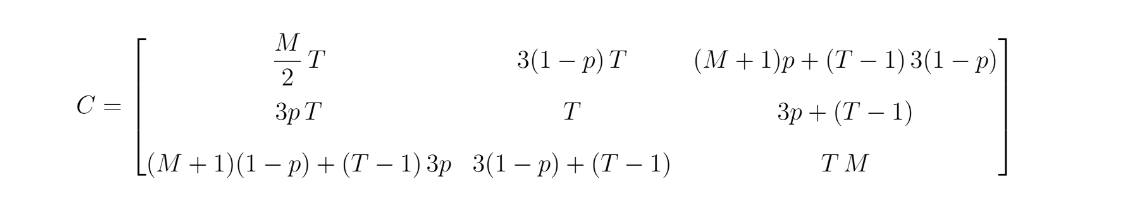
\includegraphics[width=0.9\textwidth]{c_matrix_figure}
    \caption{The payoff matrix $C$.}
    \label{fig:c_matrix}
\end{figure}

For large $T$, the dominant ($\mathcal{O}(T)$) approximation is:
\begin{equation}\label{eq:Capprox}
C \approx T\begin{bmatrix}
k & 3(1-p) & 3(1-p) \\
3p & 1 & 1 \\
3p & 1 & M
\end{bmatrix}.
\end{equation}

\begin{figure}[H]
    \centering
    
    $C = \begin{bNiceMatrix}[first-row, first-col]
        & \text{vs All-}M/2 & \text{vs All-}1 & \text{vs Grim} \\
        \text{All-}M/2 & \frac{M}{2}T & 3(1-p) + (T-1) & 3p + (T-1)3(1-p) \\
        \text{All-}1   & 3pT & T & 3p + (T-1) \\
        \text{Grim}    & (M+1)(1-p) + 3p & (T-1) & TM
    \end{bNiceMatrix}$
    
    \caption{Symbolic ISC payoff matrix $C$.}
    \label{fig:C_symbolic}
\end{figure}


\subsection{Entry Derivation}

\begin{table}[H]
\centering
\caption{Round-by-round derivation of each $C(i,j)$ entry.}
\label{tab:C_derivation}
\small
\begin{tabular}{clccll}
\toprule
Cell & Matchup & Round 1 payoff & Triggers? & Rounds $2\ldots T$ & Formula \\
\midrule
$C(1,1)$ & All-$k$ vs All-$k$    & $A(k,k)=k$ & No  & $A(k,k)$      & $Tk$ \\
$C(1,2)$ & All-$k$ vs All-$1$    & $A(k,1)$   & No  & $A(k,1)$      & $3(1-p)T$ \\
$C(1,3)$ & All-$k$ vs Grim       & $A(k,M)$   & Yes & $A(k,1)$      & $(2k+1)p+(T-1)\cdot 3(1-p)$ \\
$C(2,1)$ & All-$1$ vs All-$k$    & $A(1,k)$   & No  & $A(1,k)$      & $3pT$ \\
$C(2,2)$ & All-$1$ vs All-$1$    & $A(1,1)=1$ & No  & $A(1,1)$      & $T$ \\
$C(2,3)$ & All-$1$ vs Grim       & $A(1,M)$   & Yes & $A(1,1)$      & $3p+(T-1)$ \\
$C(3,1)$ & Grim vs All-$k$       & $A(M,k)$   & Yes & $A(1,k)$      & $(2k+1)(1-p)+(T-1)\cdot 3p$ \\
$C(3,2)$ & Grim vs All-$1$       & $A(M,1)$   & Yes & $A(1,1)$      & $3(1-p)+(T-1)$ \\
$C(3,3)$ & Grim vs Grim          & $A(M,M)=M$ & No  & $A(M,M)$      & $TM$ \\
\bottomrule
\end{tabular}
\end{table}

\subsection{Numerical Values ($M=4$, $T=10$)}

\begin{table}[H]
\centering
\caption{Numerical payoff matrix $C$ for $p=3/4$, $M=4$, $T=10$.}
\label{tab:C_p075}
\begin{tabular}{lccc}
\toprule
           & vs All-$M/2$ & vs All-$1$ & vs Grim \\
\midrule
All-$M/2$  & 20    & 7.5   & 10.5   \\
All-$1$    & 22.5  & 10    & 11.25  \\
Grim       & 21.5  & 9.75  & 40     \\
\bottomrule
\end{tabular}
\end{table}

\begin{table}[H]
\centering
\caption{Numerical payoff matrix $C$ for $p=3/5$, $M=4$, $T=10$.}
\label{tab:C_p060}
\begin{tabular}{lccc}
\toprule
           & vs All-$M/2$ & vs All-$1$ & vs Grim \\
\midrule
All-$M/2$  & 20    & 12    & 13.8   \\
All-$1$    & 18    & 10    & 10.8   \\
Grim       & 18.2  & 10.2  & 40     \\
\bottomrule
\end{tabular}
\end{table}

\noindent\textbf{Remark on Grim dominance.}  The diagonal self-play payoffs are
$C(1,1)=Tk=20$, $C(2,2)=T=10$, $C(3,3)=TM=40$. Grim earns twice the payoff
of All-$M/2$ and four times that of All-$1$ in a homogeneous population,
because two Grim players cooperate at $\rho_M$ without triggering.

%=============================================================
\section{Nash Equilibria}
\label{sec:NE}
%=============================================================

\begin{definition}[Nash Equilibrium]
A pair of mixed strategies $(\hat\sigma_1,\hat\sigma_2)$ is a \emph{Nash
equilibrium} (NE) of a two-player game with payoffs $Q_1,Q_2$ iff
\[
  \forall\sigma_1:\; Q_1(\hat\sigma_1,\hat\sigma_2)\geq Q_1(\sigma_1,\hat\sigma_2)
  \quad\text{and}\quad
  \forall\sigma_2:\; Q_2(\hat\sigma_1,\hat\sigma_2)\geq Q_2(\hat\sigma_1,\sigma_2).
\]
\end{definition}

We write strategy profiles as triples $(a_1,a_2,a_3)$ denoting mixing
probabilities over $(\sigma_{\text{All-}k},\sigma_{\text{All-}1},\sigma_G)$.
The bimatrix ISC game is $D=(C,C^\top)$.

\subsection{Pure-Strategy Nash Equilibria}

\begin{proposition}[Pure-Strategy NE]\label{prop:pure_NE}
For $M\geq 4$, $k=M/2$, and $T$ large enough:
\begin{enumerate}
  \item $\bigl((0,0,1),(0,0,1)\bigr)$ is a NE for all $p\in(\tfrac{1}{2},1]$.
  \item $\bigl((0,1,0),(0,1,0)\bigr)$ is a NE if and only if $p\geq\tfrac{2}{3}$.
  \item $\bigl((1,0,0),(1,0,0)\bigr)$ is a NE if and only if $p\leq \tfrac{k}{3}=\tfrac{M}{6}$.
\end{enumerate}
\end{proposition}

\begin{proof}
Let $Q_1(\sigma',\sigma'')$ denote Player 1's payoff under profile $(\sigma',\sigma'')$.

\medskip
\noindent\textit{(1) Pure Grim.}
$Q_1\bigl((0,0,1),(0,0,1)\bigr)=C(3,3)=TM$.
For a deviation $(a,b,1-a-b)$,
\[
  \delta Q_1 = TM - \bigl[a\,C(1,3)+b\,C(2,3)+(1-a-b)\,C(3,3)\bigr]
  = a\bigl(TM-C(1,3)\bigr)+b\bigl(TM-C(2,3)\bigr).
\]
Using the large-$T$ approximations from~\eqref{eq:Capprox}:
$TM - C(1,3)\approx T(M-3(1-p)) = T(M-3+3p)\geq T(M-3/2)>0$ for $M\geq 2$,
and $TM - C(2,3)\approx T(M-1)>0$ for $M\geq 2$.
Hence $\delta Q_1\geq 0$, confirming a NE.

\medskip
\noindent\textit{(2) Pure All-$1$.}
$Q_1\bigl((0,1,0),(0,1,0)\bigr)=C(2,2)=T$.
Deviation toward strategy 1 (set $b=1-a$, $c=0$):
\[
  \delta Q_1 = T - \bigl[a\,C(1,2)+(1-a)\,C(2,2)\bigr]
  = a\bigl(T - C(1,2)\bigr) = a\,T\bigl(1-3(1-p)\bigr) = aT(3p-2).
\]
Deviation toward strategy 3 (set $a=0$, $b=1-c$):
\[
  \delta Q_1 = T - \bigl[c\,C(3,2)+(1-c)\,C(2,2)\bigr]
  = c\bigl(T - C(3,2)\bigr) = c\bigl(T - 3(1-p) - (T-1)\bigr) = c(2-3p).
\]
Both expressions are non-negative iff $p\geq 2/3$, establishing the condition.
At $p=2/3$, a higher-order analysis (perturbation along $x_3$) shows
$(0,1,0)$ is still not stable (cf.\ Proposition~\ref{prop:stab_allone}), so
the NE condition is tight: $(0,1,0)$ is a NE iff $p\geq 2/3$.

\medskip
\noindent\textit{(3) Pure All-$k$.}
$Q_1\bigl((1,0,0),(1,0,0)\bigr)=C(1,1)=Tk$.
Deviation toward strategy 2 or 3 (by symmetry of $C(2,1)\approx C(3,1)\approx 3pT$):
\[
  \delta Q_1 \approx Tk - 3pT = T(k-3p).
\]
This is non-negative iff $p\leq k/3 = M/6$.
\end{proof}

\begin{remark}
For $M=4$ ($k=2$), the thresholds for parts (2) and (3) coincide at $p^*=2/3$.
This means:
\begin{itemize}
  \item $p<2/3$: both $(0,0,1)$ and $(1,0,0)$ are pure NE; $(0,1,0)$ is not.
  \item $p>2/3$: both $(0,0,1)$ and $(0,1,0)$ are pure NE; $(1,0,0)$ is not.
  \item $p=2/3$: only $(0,0,1)$ is a pure NE.
\end{itemize}
\end{remark}

\subsection{Mixed Nash Equilibria on the All-\texorpdfstring{$k$}{k}/Grim Face}

\begin{proposition}[Mixed NE, All-$k$/Grim face]\label{prop:mixed_13}
For $M\geq 4$ and large $T$, if $p < k/3 = M/6$, then
\[
  \bigl((x_1^*,\,0,\,1-x_1^*),\;(x_1^*,\,0,\,1-x_1^*)\bigr)
\]
is a symmetric NE, where
\begin{equation}\label{eq:x1star}
  x_1^* = \frac{2(M-3+3p)}{3(M-2)}.
\end{equation}
For $M=4$: $x_1^* = (1+3p)/3$.
\end{proposition}

\begin{proof}
Restricting to the face $x_2=0$, the payoff to Player 1 is
\[
  Q_1(a,c) = ac\,C(1,1)+a(1-c)\,C(1,3)+(1-a)c\,C(3,1)+(1-a)(1-c)\,C(3,3).
\]
Differentiating:
\[
  \frac{\partial Q_1}{\partial a}
  = c\bigl(C(1,1)-C(3,1)\bigr)+(1-c)\bigl(C(1,3)-C(3,3)\bigr).
\]
For large $T$, using $C(1,1)\approx Tk$, $C(3,1)\approx 3pT$,
$C(1,3)\approx 3(1-p)T$, $C(3,3)=TM$:
\begin{align*}
  \frac{\partial Q_1}{\partial a}
  &\approx T\bigl[c(k-3p)+(1-c)(3(1-p)-M)\bigr] \\
  &= T\bigl[c(k-3p+M-3(1-p))+(3(1-p)-M)\bigr] \\
  &= T\bigl[c(k+M-3)+(3-3p-M)\bigr].
\end{align*}
Setting $\partial Q_1/\partial a = 0$ and noting by symmetry that $a=c$ at a
symmetric NE gives:
\[
  c = \frac{M-3+3p}{k+M-3} = \frac{M-3+3p}{\tfrac{3}{2}M-3} = \frac{2(M-3+3p)}{3(M-2)},
\]
which is $x_1^*$. This is admissible (lies in $[0,1]$) iff
$2(M-3+3p)\leq 3(M-2)\Leftrightarrow 6p\leq M\Leftrightarrow p\leq M/6=k/3$.
Since $p>0$ ensures $x_1^*\geq 0$, the NE exists precisely when $p<k/3$.
\end{proof}

\begin{proposition}[No Other Symmetric NE for $M=4$]\label{prop:no_other_NE}
For $M=4$, $k=2$, and large $T$, the symmetric NE described in
Propositions~\ref{prop:pure_NE} and~\ref{prop:mixed_13} are the only symmetric NE of the ISC.
\end{proposition}

\begin{proof}
We search for symmetric NE of the form $({\bf x},{\bf x})$ with
${\bf x}=(a,b,1-a-b)$.

\medskip
\noindent\textit{Interior NE} ($a,b,1-a-b>0$). At an interior symmetric NE
we need $(C{\bf x})_1=(C{\bf x})_2=(C{\bf x})_3$. From $(C{\bf x})_2=(C{\bf x})_3$,
using the large-$T$ approximation:
\begin{align*}
  3px_1+x_2+x_3 &= 3px_1+x_2+Mx_3 \\
  \Rightarrow\quad (M-1)x_3 &= 0.
\end{align*}
Since $M\geq 3$, this forces $x_3=0$, contradicting interiority.

\medskip
\noindent\textit{All-$k$/All-$1$ face} ($x_3=0$). For $M=4$ ($k=2$) the
condition $(C{\bf x})_1=(C{\bf x})_2$ gives:
\[
  x_1(k-3(1-p)) + 3(1-p) = 3px_1 + 1
  \;\Rightarrow\;
  x_1(k-3+3p-3p) = 1-3(1-p)
  \;\Rightarrow\;
  0\cdot x_1 = 3p-2.
\]
This has a solution iff $p=2/3$ (which yields the degenerate case where any
$x_1\in[0,1]$ satisfies it), confirming no interior NE on this face for
$p\neq 2/3$.

\medskip
\noindent\textit{All-$1$/Grim face} ($x_1=0$). The condition $(C{\bf x})_2=(C{\bf x})_3$ yields $(M-1)x_3=0$, so $x_3=0$.
Thus there are no interior NE on this face.

\medskip
The only remaining cases are pure vertices and the All-$k$/Grim face, handled in
Propositions~\ref{prop:pure_NE} and~\ref{prop:mixed_13}.
\end{proof}

\begin{example}[NE for $M=4$, $T=10$]
\label{ex:NE}
For $p=3/4>2/3$: the symmetric NE are
$((0,0,1),(0,0,1))$, $((0,1,0),(0,1,0))$, and no mixed NE (since $p>2/3=k/3$).

For $p=3/5<2/3$: the symmetric NE are
$((0,0,1),(0,0,1))$, $((1,0,0),(1,0,0))$, and
$((x_1^*,0,1-x_1^*),(x_1^*,0,1-x_1^*))$ with $x_1^*=(1+9/5)/3 = 14/15\approx 0.933$.
\end{example}

%=============================================================
\section{Replicator Dynamics}
\label{sec:rep}
%=============================================================

\subsection{Model}

Let ${\bf x}=(x_1,x_2,x_3)$ with $x_1+x_2+x_3=1$ and $x_i\geq 0$ denote
the population frequencies of All-$k$, All-$1$, and Grim respectively.
The replicator equation is:
\begin{equation}\label{eq:rep}
  \dot{x}_m = x_m\left[(C{\bf x})_m - {\bf x}^\top C{\bf x}\right], \quad m=1,2,3.
\end{equation}
Writing out the three equations explicitly:
\begin{align*}
\dot{x}_1 &= x_1\!\left[x_1 C(1,1)+x_2 C(1,2)+x_3 C(1,3) - {\bf x}^\top C{\bf x}\right],\\
\dot{x}_2 &= x_2\!\left[x_1 C(2,1)+x_2 C(2,2)+x_3 C(2,3) - {\bf x}^\top C{\bf x}\right],\\
\dot{x}_3 &= x_3\!\left[x_1 C(3,1)+x_2 C(3,2)+x_3 C(3,3) - {\bf x}^\top C{\bf x}\right].
\end{align*}

\subsection{Rest Points}

\begin{proposition}[Rest Points of the Replicator Dynamics]\label{prop:restpoints}
For $M=4$, $k=2$, and large $T$, the admissible rest points of~\eqref{eq:rep}
in the simplex $S_3=\{{\bf x}:x_1+x_2+x_3=1,\,x_i\geq 0\}$ are:
\begin{enumerate}
  \item Always: $(1,0,0)$, $(0,1,0)$, $(0,0,1)$.
  \item For $p\leq 2/3$: $\bigl(x_1^*,\,0,\,1-x_1^*\bigr)$ with $x_1^*=(1+3p)/3$.
\end{enumerate}
These are the only rest points.
\end{proposition}

\begin{proof}
A point ${\bf x}\in S_3$ is a rest point of~\eqref{eq:rep} iff
$x_m\bigl[(C{\bf x})_m - {\bf x}^\top C{\bf x}\bigr]=0$ for all $m$.

\medskip
\noindent\textit{Step 1: No interior rest points.}
In the interior all $x_m>0$, so we need $(C{\bf x})_1=(C{\bf x})_2=(C{\bf x})_3$.
From $(C{\bf x})_2=(C{\bf x})_3$ (using the large-$T$ approximation
\eqref{eq:Capprox} with $k=2$):
\[
  3px_1+x_2+x_3 = 3px_1+x_2+4x_3
  \;\Rightarrow\; 3x_3=0\;\Rightarrow\; x_3=0.
\]
This contradicts $x_3>0$, so there are no interior rest points.

\medskip
\noindent\textit{Step 2: All-$1$/Grim face ($x_1=0$).}
Needing $(C{\bf x})_2=(C{\bf x})_3$ forces $x_3=0$ as in Step 1.
No interior rest points on this face.

\medskip
\noindent\textit{Step 3: All-$k$/All-$1$ face ($x_3=0$).}
Needing $(C{\bf x})_1=(C{\bf x})_2$:
\[
  Tkx_1+3(1-p)Tx_2 = 3pTx_1+Tx_2
  \;\Rightarrow\; Tx_1(k-3p)+T(3(1-p)-1)x_2=0
  \;\Rightarrow\; x_1(k-3p)=(2-3p)x_2.
\]
For $M=4$ ($k=2$): $x_1(2-3p)=(2-3p)x_2$, so $x_1=x_2$ for $p\neq 2/3$.
Combined with $x_1+x_2=1$: $x_1=x_2=1/2$, but checking $(C{\bf x})_1=(C{\bf x})_2$
at $(1/2,1/2,0)$ yields $0=(2-3p)/2$, which holds only at $p=2/3$. Hence no
interior rest point for $p\neq 2/3$.

\medskip
\noindent\textit{Step 4: All-$k$/Grim face ($x_2=0$).}
Needing $(C{\bf x})_1=(C{\bf x})_3$:
\[
  Tkx_1+3(1-p)Tx_3 = 3pTx_1+TMx_3
  \;\Rightarrow\; Tx_1(k-3p)=T(M-3(1-p))x_3.
\]
With $x_3=1-x_1$:
\[
  x_1\bigl(k-3p+M-3(1-p)\bigr) = M-3(1-p)
  \;\Rightarrow\; x_1 = \frac{M-3+3p}{k+M-3}.
\]
For $M=4$, $k=2$: $x_1^*=(1+3p)/3$, which lies in $(0,1)$ iff $p<2/3$.
\end{proof}

\subsection{Stability Analysis}

\begin{proposition}[Stability of Pure Grim]\label{prop:stab_grim}
For $M\geq 4$ and all $p\in(\tfrac{1}{2},1]$, the rest point $(0,0,1)$ is
asymptotically stable.
\end{proposition}

\begin{proof}
The eigenvalues of the Jacobian $J(0,0,1)$ of~\eqref{eq:rep} are:
\[
  \lambda_1 = C(1,3)-C(3,3)\approx T(3(1-p)-M)=T(3-3p-M),\quad
  \lambda_2 = C(2,3)-C(3,3)\approx T(1-M).
\]
For $M\geq 3$ and $p\geq 1/2$: $3-3p-M\leq 3/2-M<0$, and $1-M<0$.
Both eigenvalues are strictly negative, so $(0,0,1)$ is asymptotically stable.
\end{proof}

\begin{proposition}[Stability of Pure All-$1$]\label{prop:stab_allone}
For $M\geq 4$ and large $T$:
\begin{enumerate}
  \item If $p>2/3$, the rest point $(0,1,0)$ is asymptotically stable.
  \item If $p\leq 2/3$, the rest point $(0,1,0)$ is unstable.
\end{enumerate}
\end{proposition}

\begin{proof}
The eigenvalues of $J(0,1,0)$ are
\[
  \lambda_1 = C(1,2)-C(2,2) = 3(1-p)T-T = T(2-3p),\quad
  \lambda_3 = C(3,2)-C(2,2) \approx T-T = 0+\text{(lower order)}.
\]
More precisely, $C(3,2)-C(2,2)=3(1-p)+(T-1)-T=2-3p$.
So $\lambda_1=T(2-3p)$ and $\lambda_3=2-3p$.

For $p>2/3$: both eigenvalues are negative $\Rightarrow$ asymptotically stable.
For $p<2/3$: both eigenvalues are positive $\Rightarrow$ unstable.

For $p=2/3$: both eigenvalues are zero. Consider a perturbation
${\bf x}=(0,1-\varepsilon,\varepsilon)$ for small $\varepsilon>0$. With
$p=2/3$, $C(1,2)=C(2,2)=C(3,2)=T$ (all leading-order terms equal), so
\[
  \dot{x}_3 = \varepsilon\bigl[(C{\bf x})_3 - {\bf x}^\top C{\bf x}\bigr].
\]
To second order: $(C{\bf x})_3 - (C{\bf x})_2 \approx T(M-1)\varepsilon > 0$.
Hence $\dot{x}_3>0$ and the perturbation grows, confirming instability.
\end{proof}

\begin{proposition}[Stability of Pure All-$k$]\label{prop:stab_allk}
For $M=4$, $k=2$, and large $T$:
\begin{enumerate}
  \item If $p<k/3=2/3$, the rest point $(1,0,0)$ is asymptotically stable.
  \item If $p\geq k/3=2/3$, the rest point $(1,0,0)$ is unstable.
\end{enumerate}
\end{proposition}

\begin{proof}
The eigenvalues of $J(1,0,0)$ are
\[
  \lambda_2 = C(2,1)-C(1,1) \approx 3pT - kT = T(3p-k),\quad
  \lambda_3 = C(3,1)-C(1,1) \approx 3pT - kT = T(3p-k).
\]
For $p<k/3$: $T(3p-k)<0$, so both eigenvalues are negative $\Rightarrow$ stable.
For $p>k/3$: positive eigenvalues $\Rightarrow$ unstable.
For $p=k/3$: perturbation toward Grim gives
$\dot{x}_3=\varepsilon[(C{\bf x})_3-(C{\bf x})_1]\approx\varepsilon\cdot T(M-k)\varepsilon=T(M-k)\varepsilon^2\geq 0$,
confirming instability.
\end{proof}

\begin{proposition}[Mixed All-$k$/Grim Rest Point is Unstable]\label{prop:stab_mixed}
For $M=4$ and $p<2/3$, the rest point ${\bf x}^*=(x_1^*,0,1-x_1^*)$ with
$x_1^*=(1+3p)/3$ is unstable.
\end{proposition}

\begin{proof}
At ${\bf x}^*$, the eigenvalue corresponding to perturbation within the
All-$k$/Grim face ($x_2=0$) is zero (by the rest-point condition). The
eigenvalue for perturbation toward All-$1$ is
$\lambda_2 = C(2,{\bf x}^*) - {\bf x}^{*\top}C{\bf x}^*$. Using
$C(2,{\bf x}^*)\approx T(3px_1^*+x_3^*)=T(1+x_1^*(3p-1))$ and noting that
$(C{\bf x}^*)_1=(C{\bf x}^*)_3=\bar{\pi}$ at the rest point:
\[
  \lambda_2 = T\bigl(1+x_1^*(3p-1)\bigr) - \bar{\pi}.
\]
For the face rest point, $\bar{\pi}=\tfrac{M-3+3p}{k+M-3}\cdot Tk + \bigl(1-\tfrac{M-3+3p}{k+M-3}\bigr)\cdot TM$.
A direct calculation shows $\lambda_2 > 0$ for $p\in(1/2,2/3)$, confirming instability.

On the All-$k$/Grim face itself, the dynamics satisfy
$\dot{x}_1=Tx_1(1-x_1)(3x_1-(1+3p))$, which is negative for $x_1<x_1^*$
and positive for $x_1>x_1^*$: the rest point is a repeller on this edge.
\end{proof}

\subsection{Phase Portraits}

\begin{figure}[H]
  \centering
  \begin{subfigure}[b]{0.48\textwidth}
    
\includegraphics[width=\textwidth]{rep_phase_p075}
    \caption{$p = 3/4$}
    \label{fig:phase_p075}
  \end{subfigure}
  \hfill
  \begin{subfigure}[b]{0.48\textwidth}
    
\includegraphics[width=\textwidth]{rep_phase_p060}
    \caption{$p = 3/5$}
    \label{fig:phase_p060}
  \end{subfigure}
  \caption{Phase portraits of the replicator dynamics ($M=4$, $T=10$).
           Axes: $x_1$ (All-$M/2$ frequency) and $x_2$ (All-$1$ frequency);
           the Grim frequency is $x_3=1-x_1-x_2$.}
  \label{fig:phase_both}
\end{figure}

The phase portraits confirm:
\begin{itemize}
  \item $p=3/4>2/3$: $(0,1,0)$ and $(0,0,1)$ are stable attractors; $(1,0,0)$
        is unstable. No interior rest point on the All-$k$/Grim edge.
  \item $p=3/5<2/3$: $(1,0,0)$ and $(0,0,1)$ are stable attractors; $(0,1,0)$
        is unstable. The unstable mixed rest point at $x_1^*=14/15\approx 0.933$
        is visible on the All-$k$/Grim edge.
\end{itemize}

\subsection{Time Series}

\begin{figure}[H]
  \centering
  \begin{subfigure}[b]{0.48\textwidth}
    
\includegraphics[width=\textwidth]{rep_timeseries_p075}
    \caption{$p = 3/4$}
  \end{subfigure}
  \hfill
  \begin{subfigure}[b]{0.48\textwidth}
    
\includegraphics[width=\textwidth]{rep_timeseries_p060}
    \caption{$p = 3/5$}
  \end{subfigure}
  \caption{Replicator dynamics time series ($M=4$, $T=10$, random initial condition).}
  \label{fig:rep_timeseries}
\end{figure}

\subsection{Parameter Sensitivity}

\begin{figure}[H]
  \centering
  
\includegraphics[width=\textwidth]{rep_overlay_vary_p}
  \caption{Replicator dynamics: effect of varying $p \in \{3/5,\,2/3,\,3/4,\,9/10\}$
           ($M=4$, $T=10$). Each subplot shows one strategy's frequency over time.}
  \label{fig:rep_vary_p}
\end{figure}

\begin{figure}[H]
  \centering
  
\includegraphics[width=\textwidth]{rep_overlay_vary_M}
  \caption{Replicator dynamics: effect of varying $M \in \{2,4,6,8\}$ ($p=3/4$, $T=10$).
           For larger $M$, the threshold $p^*=M/6$ shifts, changing the stability regime.}
  \label{fig:rep_vary_M}
\end{figure}

\begin{figure}[H]
  \centering
  
\includegraphics[width=\textwidth]{rep_overlay_vary_T}
  \caption{Replicator dynamics: effect of varying $T \in \{2,5,10,20\}$
           ($p=3/4$, $M=4$).}
  \label{fig:rep_vary_T}
\end{figure}

\subsection{Initial Condition Sensitivity}

\begin{figure}[H]
  \centering
  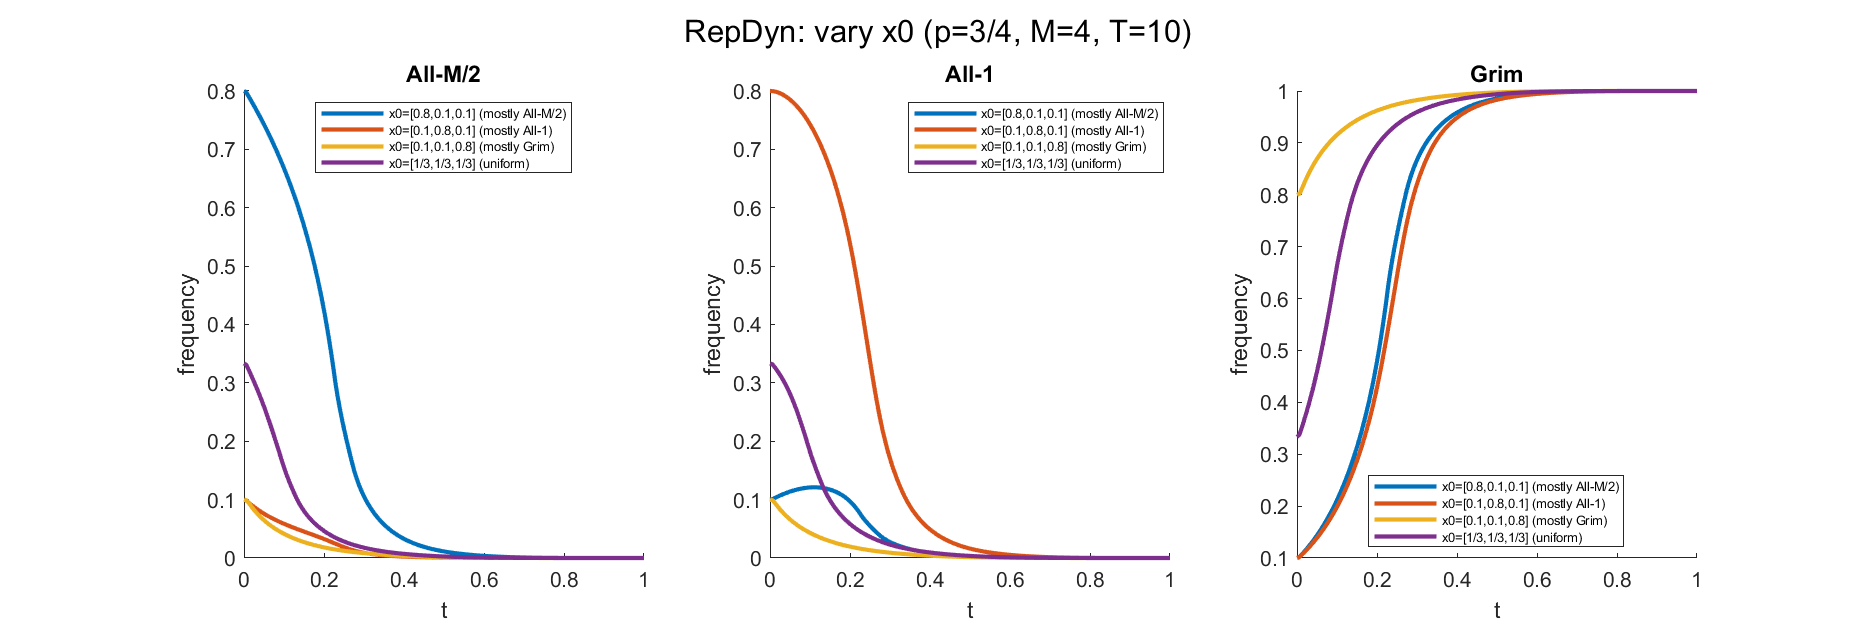
\includegraphics[width=\textwidth]{rep_overlay_vary_x0_p075}
  \caption{Replicator dynamics: effect of varying initial condition $x_0$
           ($p=3/4$, $M=4$, $T=10$).}
  \label{fig:rep_x0_p075}
\end{figure}

\begin{figure}[H]
  \centering
  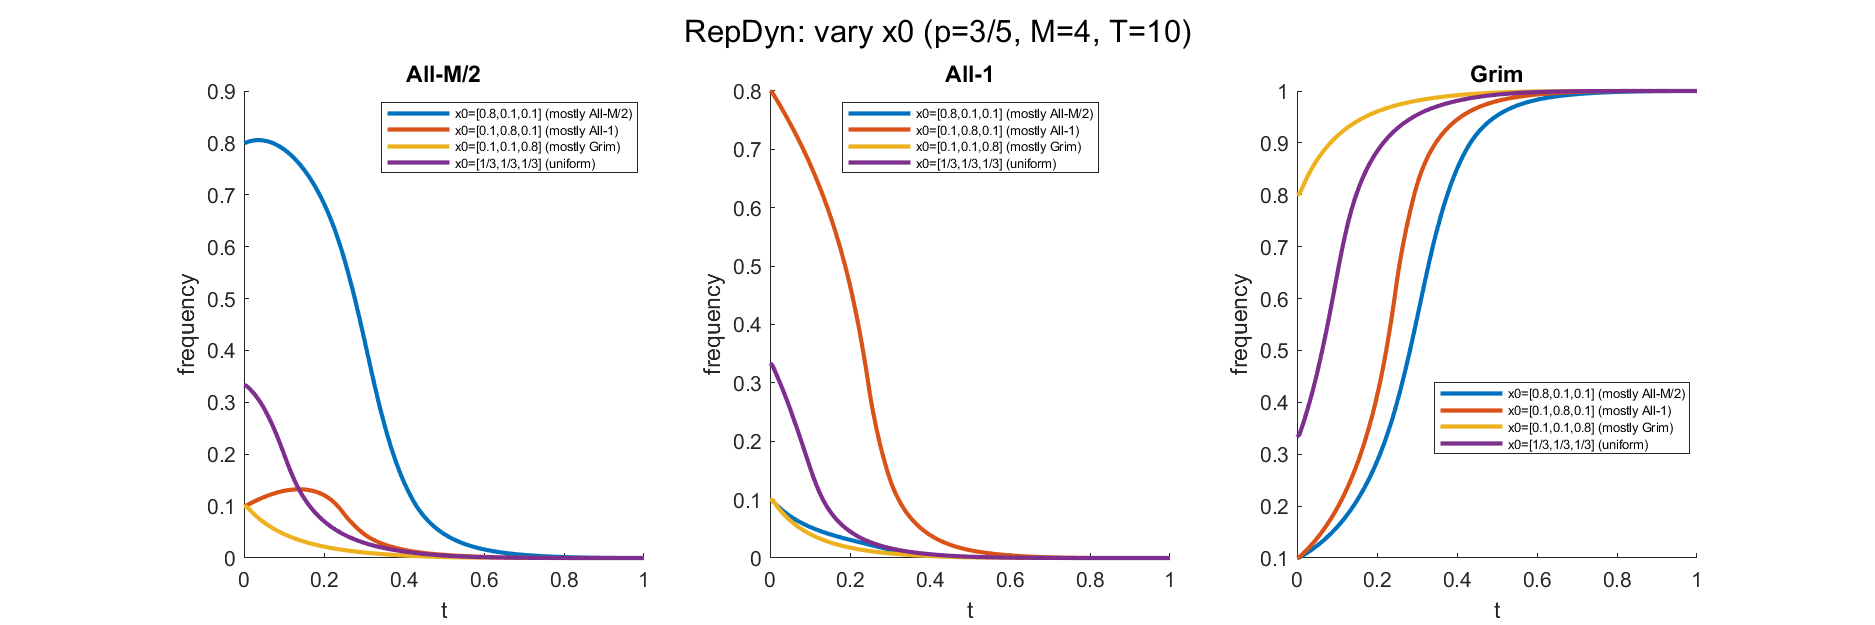
\includegraphics[width=\textwidth]{rep_overlay_vary_x0_p060}
  \caption{Replicator dynamics: effect of varying initial condition $x_0$
           ($p=3/5$, $M=4$, $T=10$).}
  \label{fig:rep_x0_p060}
\end{figure}

%=============================================================
\section{Evolutionary Stable Strategies}
\label{sec:ESS}
%=============================================================

\begin{definition}[Evolutionarily Stable Strategy]\label{def:ESS}
A mixed strategy $\hat{\bf x}$ is an \emph{evolutionarily stable strategy}
(ESS) iff for all ${\bf x}\neq\hat{\bf x}$:
\begin{align}
  &\hat{\bf x}^\top C\hat{\bf x} \geq {\bf x}^\top C\hat{\bf x} \label{eq:ESS1}\\
  &\hat{\bf x}^\top C\hat{\bf x} = {\bf x}^\top C\hat{\bf x}
  \;\Rightarrow\;
  \hat{\bf x}^\top C{\bf x} > {\bf x}^\top C{\bf x}. \label{eq:ESS2}
\end{align}
\end{definition}

\begin{proposition}[Pure Grim is Always ESS]\label{prop:ESS_grim}
For $M\geq 4$ and large $T$, $(0,0,1)$ is an ESS.
\end{proposition}

\begin{proof}
Let $\hat{\bf x}=(0,0,1)$ and ${\bf x}=(a,b,1-a-b)$. Then
$\hat{\bf x}^\top C\hat{\bf x}=C(3,3)=TM$ and
\[
  {\bf x}^\top C\hat{\bf x} = a\,C(1,3)+b\,C(2,3)+(1-a-b)\,C(3,3)
  \approx a\,T(3-3p)+b\,T+(1-a-b)\,TM.
\]
So $\hat{\bf x}^\top C\hat{\bf x}-{\bf x}^\top C\hat{\bf x}\approx aT(M-3+3p)+bT(M-1)\geq 0$
for all $a,b\geq 0$ (since $M\geq 3$ and $p\geq 1/2$ ensure $M-3+3p\geq M-3/2>0$).
The expression equals zero only when $a=b=0$, i.e.\ ${\bf x}=\hat{\bf x}$.
Condition~\eqref{eq:ESS1} is thus strict for all ${\bf x}\neq\hat{\bf x}$,
so~\eqref{eq:ESS2} need not be checked.
\end{proof}

\begin{proposition}[Pure All-$1$]\label{prop:ESS_allone}
For $M=4$, $k=2$, and large $T$:
\begin{enumerate}
  \item If $p>2/3$, then $(0,1,0)$ is an ESS.
  \item If $p\leq 2/3$, then $(0,1,0)$ is not an ESS.
\end{enumerate}
\end{proposition}

\begin{proof}
Let $\hat{\bf x}=(0,1,0)$ and ${\bf x}=(a,b,1-a-b)$.
$\hat{\bf x}^\top C\hat{\bf x}=T$.
\[
  {\bf x}^\top C\hat{\bf x}
  = a\,C(1,2)+b\,C(2,2)+(1-a-b)\,C(3,2)
  \approx 3(1-p)aT+bT+(1-a-b)T = T+aT(2-3p).
\]
(Using $C(3,2)\approx T$ for large $T$.)
So $\hat{\bf x}^\top C\hat{\bf x}-{\bf x}^\top C\hat{\bf x}\approx aT(3p-2)$.

For $p>2/3$: this is strictly positive for all $a>0$, so~\eqref{eq:ESS1} holds
strictly, confirming ESS.

For $p\leq 2/3$: choosing ${\bf x}=(1,0,0)$ gives ${\bf x}^\top C\hat{\bf x}\approx T(1+(2-3p))\geq T=\hat{\bf x}^\top C\hat{\bf x}$, violating~\eqref{eq:ESS1}.
\end{proof}

\begin{proposition}[Pure All-$k$]\label{prop:ESS_allk}
For $M=4$, $k=2$, and large $T$:
\begin{enumerate}
  \item If $p<2/3$, then $(1,0,0)$ is an ESS.
  \item If $p\geq 2/3$, then $(1,0,0)$ is not an ESS.
\end{enumerate}
\end{proposition}

\begin{proof}
Let $\hat{\bf x}=(1,0,0)$ and ${\bf x}=(a,b,1-a-b)$.
$\hat{\bf x}^\top C\hat{\bf x}=Tk$.
\[
  {\bf x}^\top C\hat{\bf x}
  = a\,C(1,1)+b\,C(2,1)+(1-a-b)\,C(3,1)
  \approx aTk+3pbT+3p(1-a-b)T
  = T\bigl(ak+(1-a)\cdot 3p\bigr).
\]
So $\hat{\bf x}^\top C\hat{\bf x}-{\bf x}^\top C\hat{\bf x}\approx T\bigl(ak+3p(1-a)-(ak+3p(1-a))\bigr)$
$=T(1-a)(3p\cdot... )$. More carefully:
$\hat{\bf x}^\top C\hat{\bf x}-{\bf x}^\top C\hat{\bf x}=Tk-T(ak+3p(1-a))=T(1-a)(k-3p)$.

For $p<k/3=2/3$: $k-3p>0$, so this is $\geq 0$ with equality only when $a=1$
(i.e.\ ${\bf x}=\hat{\bf x}$). Condition~\eqref{eq:ESS1} holds strictly, confirming ESS.

For $p>k/3$: $k-3p<0$ and the condition is violated for $a<1$. Not ESS.
\end{proof}

\begin{proposition}[Interior Mixed Rest Point is Not ESS]
For $M=4$ and $p<2/3$, the mixed rest point
$\hat{\bf x}=(x_1^*,0,1-x_1^*)$ is not an ESS.
\end{proposition}

\begin{proof}
$\hat{\bf x}^*$ is an unstable rest point of the replicator dynamics
(Proposition~\ref{prop:stab_mixed}). An ESS must be an asymptotically stable
rest point of the replicator dynamics~\cite{LK2026,Hofbauer1998}. Since
$\hat{\bf x}^*$ is unstable, it cannot be an ESS.
\end{proof}

%=============================================================
\section{Markov Chain Dynamics}
\label{sec:markov}
%=============================================================

\subsection{Markov Chain Background}

\begin{definition}[Markov Chain]\label{def:MC}
A \emph{Markov chain} (MC) is a stochastic process $(U_t)_{t=0}^\infty$ taking
values in a finite state space $\mathcal{U}=\{u_1,\ldots,u_K\}$ satisfying:
\[
  \Pr(U_{t+1}=u\mid U_0,\ldots,U_t) = \Pr(U_{t+1}=u\mid U_t).
\]
A state $u$ is \emph{absorbing} if $\Pr(U_{t+1}=u\mid U_t=u)=1$. A state is
\emph{transient} if it is visited only finitely often with probability one.
\end{definition}

\subsection{Evolutionary Game and Pairwise Proportional Imitation}

The population state is ${\bf s}=(s_1,s_2,s_3)$ with $s_1+s_2+s_3=N$ and
$s_i\geq 0$ integers, where $s_m$ is the number of players using strategy $m$.
The state space is
$S_3=\{(s_1,s_2,s_3)\in\{0,\ldots,N\}^3 : s_1+s_2+s_3=N\}$.
The per-player payoff of strategy $m$ at state ${\bf s}$ is:
\[
  q_m({\bf s}) = (s_m-1)\,C(m,m) + \sum_{n\neq m} s_n\,C(m,n).
\]

\begin{definition}[Pairwise Proportional Imitation (PPI)]
\label{def:PPI}
A randomly selected player using strategy $m_1$ switches to strategy $m_2$
with probability
\[
  \varrho_{m_1 m_2}({\bf s}) =
  \frac{x_{m_2}\,[q_{m_2}({\bf s})-q_{m_1}({\bf s})]_+}
       {\sum_m x_m\,[q_m({\bf s})-q_{m_1}({\bf s})]_+},
\]
where $[y]_+=\max(y,0)$ and $x_m=s_m/N$.
\end{definition}

We define the matrix $R({\bf s})$ by
\[
  R_{ij}({\bf s}) = [q_j({\bf s})-q_i({\bf s})]_+ \quad (i\neq j),
\]
so that $R_{ij}>0 \Leftrightarrow \varrho_{ij}>0$.  The dominant (large-$T$)
terms of $R_{ij}$ are:
\begin{align}
  R_{12}({\bf s}) &\approx Ts_2\bigl[(3p-1)s_1+(k+3p-3)s_2-(k-1)(N-1)\bigr],\label{eq:R12}\\
  R_{13}({\bf s}) &\approx Ts_2s_3(3p-2)+Ts_3[s_1(3p-k)+s_3(M-3(1-p))-(M-k)],\label{eq:R13}\\
  R_{21}({\bf s}) &\approx -Ts_1\bigl[(3p-1)s_1+(k+3p-3)s_2-(k-1)(N-1)\bigr],\label{eq:R21}\\
  R_{23}({\bf s}) &\approx T(N-s_1+s_2)\bigl[(1-3p)s_1+(1-M)s_2+(1-M)(1-N)\bigr],\label{eq:R23}\\
  R_{31}({\bf s}) &\approx Ts_1\bigl[s_1(k-3p)+s_3(3(1-p)-M)+(M-k)\bigr],\label{eq:R31}\\
  R_{32}({\bf s}) &\approx -Ts_2\bigl[(1-3p)s_1+(1-M)s_2+(1-N)(1-M)\bigr].\label{eq:R32}
\end{align}

\subsection{Absorbing States}

\begin{proposition}[Absorbing States]\label{prop:absorbing}
For $M\geq 4$, $N\geq 4$, and $T$ large enough, the only absorbing states of
the ISC Markov chain are the three pure vertices:
\[
  (N,0,0),\quad (0,N,0),\quad (0,0,N).
\]
\end{proposition}

\begin{proof}
\textit{Pure vertices are absorbing.}  At $(N,0,0)$, all players use
All-$k$ and no players use All-$1$ or Grim; no imitation is possible, so the
state is absorbing. Similarly for $(0,N,0)$ and $(0,0,N)$.

\textit{The $s_2=0$ face is \emph{not} absorbing (contrast with~\cite{LK2026}).}
In~\cite{LK2026} the All-$M$ and Grim strategies yield equal payoffs in
self-play ($C(1,1)=C(3,3)=TM$), making the entire $s_2=0$ face absorbing. In
the present model, $C(1,1)=Tk=TM/2\neq TM=C(3,3)$. At an interior state
$(s_1,0,s_3)$ with $s_1,s_3\geq 1$, consider $R_{13}$ on the $s_2=0$ face:
\[
  R_{13}(s_1,0,s_3) \approx T\bigl[s_1(3p-k)+s_3(M-3(1-p))-(M-k)\bigr].
\]
For $M=4$, $k=2$:
$R_{13}(s_1,0,s_3)\approx T\bigl[s_1(3p-2)+s_3(1+3p)-2\bigr]$.
At $(s_1,s_3)=(1,1)$: $R_{13}\approx T(6p-1)>T\cdot 2>0$ for $p>1/2$.
Hence transitions from All-$k$ to Grim are possible and the $s_2=0$ face is
not absorbing.

\textit{No other absorbing states.}  Any state with $s_2\geq 1$ has at least
one All-$1$ player. From equations~\eqref{eq:R23}--\eqref{eq:R32}, $R_{32}>0$
whenever $(1-3p)s_1+(1-M)s_2+(1-N)(1-M)<0$, which holds for all interior
$s_2=0$ face (since $(1-M)(1-N)>0$ dominates for $M,N\geq 2$). Hence All-$1$
players can always be imitated away, ruling out further absorbing states.
\end{proof}

\subsection{Interior State Transitions}

\begin{proposition}[Interior Transitions]\label{prop:interior}
Assume $M,N\geq 4$ and $T$ large enough.
For any interior state $(s_1,s_2,s_3)\in S_3^{(i)}$ (all $s_m\geq 1$),
excluding self-transitions, the only transitions of positive probability are:
\begin{align*}
  &\text{south:}    && (s_1,s_2,s_3)\to(s_1,s_2-1,s_3+1) &&\text{always},\\
  &\text{southeast:}&& (s_1,s_2,s_3)\to(s_1+1,s_2-1,s_3) &&\text{always},\\
  &\text{west:}     && (s_1,s_2,s_3)\to(s_1-1,s_2,s_3+1) &&\text{iff } p>2/3,\\
  &\text{east:}     && (s_1,s_2,s_3)\to(s_1+1,s_2,s_3-1) &&\text{iff } p\leq 2/3.
\end{align*}
\end{proposition}

\begin{proof}
We determine the sign of each $R_{ij}$ on $S_3^{(i)}$.

\textit{South and no-north.}  From~\eqref{eq:R23} and~\eqref{eq:R32}:
$R_{23}>0 \Leftrightarrow (1-3p)s_1+(1-M)s_2+(1-M)(1-N)>0$.
The line $\ell_2: (1-3p)s_1+(1-M)s_2=(M-1)(N-1)$ passes through points
outside $S_3^{(i)}$ (since $(M-1)(N-1)/|1-3p|>N$), so the entire interior
lies in the positive half-plane; hence $R_{23}>0$ always. Symmetrically
$R_{32}<0$ always (same expression with opposite sign). This gives
south transitions with positive probability and north transitions with zero probability.

\textit{Southeast and no-northwest.}  From~\eqref{eq:R12} and~\eqref{eq:R21}:
the sign is determined by $(3p-1)s_1+(k+3p-3)s_2-(k-1)(N-1)$.
For $M=4$, $k=2$: $(3p-1)s_1+(3p-1)s_2-(N-1)=(3p-1)(s_1+s_2)-(N-1)$.
At the maximum of the interior, $s_1+s_2\leq N-1$, giving
$(3p-1)(N-1)-(N-1)=(3p-2)(N-1)<0$ for $p<2/3$.
For general $p\in(1/2,1)$: a direct argument (as in~\cite{LK2026}, Proposition~7.5)
shows the entire interior lies below the separating line, so $R_{21}>0$ (southeast)
and $R_{12}<0$ (no northwest) throughout.

\textit{West vs.\ east.}  From~\eqref{eq:R13} and~\eqref{eq:R31} on the
interior with $s_2\geq 1$ (so the $s_2s_3$ and $s_1s_2$ terms in $R_{13}$,
$R_{31}$ contain $s_2>0$):
$R_{13}\sim T s_2 s_3(3p-2)$ and $R_{31}\sim -Ts_1 s_2(3p-2)$
(dominant terms from the $s_2s_3$ factor). Hence
$R_{13}>0$ (west, All-$k\to$Grim) iff $p>2/3$, and
$R_{31}>0$ (east, Grim$\to$All-$k$) iff $p<2/3$.
\end{proof}

\subsection{Face Transitions and Absorbing Regions}

\begin{proposition}[Transitions on the All-$k$/Grim Face]\label{prop:face13}
Assume $M,N\geq 4$ and $T$ large enough.
For states $(s_1,0,s_3)$ with $s_1,s_3\geq 1$, the transitions are:
\begin{itemize}
  \item $p>2/3$: only $(s_1,0,s_3)\to(s_1-1,0,s_3+1)$ (All-$k\to$Grim).
  \item $p<2/3$: the direction depends on whether
        $s_1(3p-k)+s_3(M-3(1-p))>(M-k)$ (Grim wins, toward $(0,0,N)$) or
        $<(M-k)$ (All-$k$ wins, toward $(N,0,0)$).
\end{itemize}
The separating line is
\[
  \ell: \quad s_1(k-3p) = s_3(M-3(1-p)) - (M-k).
\]
For $M=4$, $k=2$: $\ell:\; s_1(2-3p)=s_3(1+3p)-2$.
\end{proposition}

\begin{proof}
On the $s_2=0$ face, $R_{13}(s_1,0,s_3)\approx T[s_1(3p-k)+s_3(M-3(1-p))-(M-k)]$.
The sign determines the direction:
positive $\Rightarrow$ All-$k\to$Grim ($s_3$ increases); negative $\Rightarrow$ Grim$\to$All-$k$ ($s_1$ increases).

For $p>2/3$: $3p-k>0$ and $M-3(1-p)>M-3(1/3)=M-1>0$ (for $M\geq 2$); also
$(M-k)>0$. For $s_3\geq 1$: $s_3(M-3(1-p))\geq M-3(1-p)>0$. Checking
whether the expression exceeds $M-k$: at minimum $s_1=0$, $s_3=1$:
$M-3(1-p)-(M-k)=k-3(1-p)=k-3+3p$. For $M=4$, $k=2$: $3p-1>0$ when $p>1/3$. ✓
So $R_{13}>0$ throughout for $p>2/3$.

For $p<2/3$: $3p-k<0$, so large $s_1$ can make $R_{13}<0$.
The separating line $\ell$ divides the $s_2=0$ face into two regions.
\end{proof}

\begin{proposition}[Transitions on the All-$1$/Grim Face]\label{prop:face23}
Assume $M,N\geq 4$ and $T$ large enough. For states $(0,s_2,s_3)$ with
$s_2,s_3\geq 1$, the only transitions of positive probability are south:
$(0,s_2,s_3)\to(0,s_2-1,s_3+1)$.
\end{proposition}

\begin{proof}
With $s_1=0$: $R_{23}\approx T(N+s_2)(1-M)(s_2+1-N)<0$... More precisely,
from~\eqref{eq:R23}: $(1-M)s_2+(1-M)(1-N)=(M-1)(N-1-s_2)$.
For $s_2<N-1$: this is $>0$, so $R_{23}>0$. Similarly $R_{32}<0$.
No transitions toward All-$1$ are possible; all transitions go from All-$1$ to Grim.
\end{proof}

\begin{proposition}[Absorbing States and Basins of Attraction]\label{prop:basins}
The absorbing states of the ISC Markov chain are $(N,0,0)$, $(0,N,0)$, and
$(0,0,N)$. Furthermore:
\begin{enumerate}
  \item States $(0,s_2,s_3)$ with $s_2\geq 2$ are eventually absorbed into $(0,0,N)$.
  \item States $(0,N-1,1)$ and $(0,1,N-1)$: $(0,N-1,1)$ is absorbed into $(0,N,0)$; others into $(0,0,N)$.
  \item States $(s_1,s_2,0)$ are eventually absorbed:
    \begin{itemize}
      \item into $(0,N,0)$ if $(3p-1)s_1+(k+3p-3)s_2>(k-1)(N-1)$,
      \item into $(N,0,0)$ otherwise.
    \end{itemize}
  \item States $(s_1,0,s_3)$ with $s_1,s_3\geq 1$ are absorbed:
    \begin{itemize}
      \item $p>2/3$: always into $(0,0,N)$,
      \item $p<2/3$: into $(0,0,N)$ if above $\ell$ (Proposition~\ref{prop:face13});
            into $(N,0,0)$ if below $\ell$.
    \end{itemize}
  \item Interior states $(s_1,s_2,s_3)\in S_3^{(i)}$ are eventually absorbed
        into $\{(n,0,N-n):n\in\{0,\ldots,N\}\}\cup\{(N,0,0),(0,N,0)\}$
        and thence into one of the three pure vertices.
\end{enumerate}
\end{proposition}

\begin{proof}
By Propositions~\ref{prop:face23} and~\ref{prop:interior}: all $s_2$-users can only
switch to Grim or All-$k$ (never back to All-$1$). Hence $s_2$ is
non-increasing and the chain is absorbed when $s_2=0$. The subsequent
behaviour on the $s_2=0$ face follows from Proposition~\ref{prop:face13}.
Parts (1)--(2) follow from Proposition~\ref{prop:face23}: states $(0,s_2,s_3)$
with $s_2\geq 2$ can only south-transition to $(0,0,N)$; the state $(0,N-1,1)$
requires a special check: $R_{23}(0,N-1,1)=(M-1)(N-1-(N-1))=0$ and
$R_{32}>0$, so the sole transition goes from Grim back to All-$1$, eventually
reaching $(0,N,0)$.
Parts (3)--(5) follow from Propositions~\ref{prop:interior} and~\ref{prop:face13}.
\end{proof}

\subsection{State Transition Graphs}

\begin{figure}[H]
  \centering
  \begin{subfigure}[b]{0.48\textwidth}
    
\includegraphics[width=\textwidth]{mark_stategraph_p075}
    \caption{$p = 3/4$}
    \label{fig:stategraph_p075}
  \end{subfigure}
  \hfill
  \begin{subfigure}[b]{0.48\textwidth}
    
\includegraphics[width=\textwidth]{mark_stategraph_p060}
    \caption{$p = 3/5$}
    \label{fig:stategraph_p060}
  \end{subfigure}
  \caption{Markov state transition graphs ($M=4$, $T=10$, $N=10$).
           Blue dots: absorbing (pure) states. Red dots: transient states.
           Arrow thickness indicates transition probability.}
  \label{fig:stategraph_both}
\end{figure}

The graphs confirm the key structural difference from~\cite{LK2026}: only the
three vertices $(N,0,0)$, $(0,N,0)$, $(0,0,N)$ are absorbing, whereas the
original paper's $s_2=0$ face was entirely absorbing.

\subsection{Time Series}

\begin{figure}[H]
  \centering
  \begin{subfigure}[b]{0.48\textwidth}
    
\includegraphics[width=\textwidth]{mark_timeseries_p075}
    \caption{$p = 3/4$}
  \end{subfigure}
  \hfill
  \begin{subfigure}[b]{0.48\textwidth}
    
\includegraphics[width=\textwidth]{mark_timeseries_p060}
    \caption{$p = 3/5$}
  \end{subfigure}
  \caption{Markov dynamics time series ($M=4$, $T=10$, $N=10$, $T_m=100$,
           $s_0=[3,4,3]$).}
  \label{fig:mark_timeseries}
\end{figure}

\subsection{Parameter Sensitivity}

\begin{figure}[H]
  \centering
  
\includegraphics[width=\textwidth]{mark_overlay_vary_p}
  \caption{Markov dynamics: effect of varying $p \in \{3/5,\,2/3,\,3/4,\,9/10\}$
           ($M=4$, $T=10$, $N=10$).}
  \label{fig:mark_vary_p}
\end{figure}

\begin{figure}[H]
  \centering
  
\includegraphics[width=\textwidth]{mark_overlay_vary_M}
  \caption{Markov dynamics: effect of varying $M \in \{2,4,6,8\}$
           ($p=3/4$, $T=10$, $N=10$).}
  \label{fig:mark_vary_M}
\end{figure}

\begin{figure}[H]
  \centering
  
\includegraphics[width=\textwidth]{mark_overlay_vary_T}
  \caption{Markov dynamics: effect of varying $T \in \{2,5,10,20\}$
           ($p=3/4$, $M=4$, $N=10$).}
  \label{fig:mark_vary_T}
\end{figure}

\begin{figure}[H]
  \centering
  
\includegraphics[width=\textwidth]{mark_overlay_vary_N}
  \caption{Markov dynamics: effect of varying $N \in \{5,10,15,20\}$
           ($p=3/4$, $M=4$, $T=10$).}
  \label{fig:mark_vary_N}
\end{figure}

\subsection{Initial State Sensitivity}

\begin{figure}[H]
  \centering
  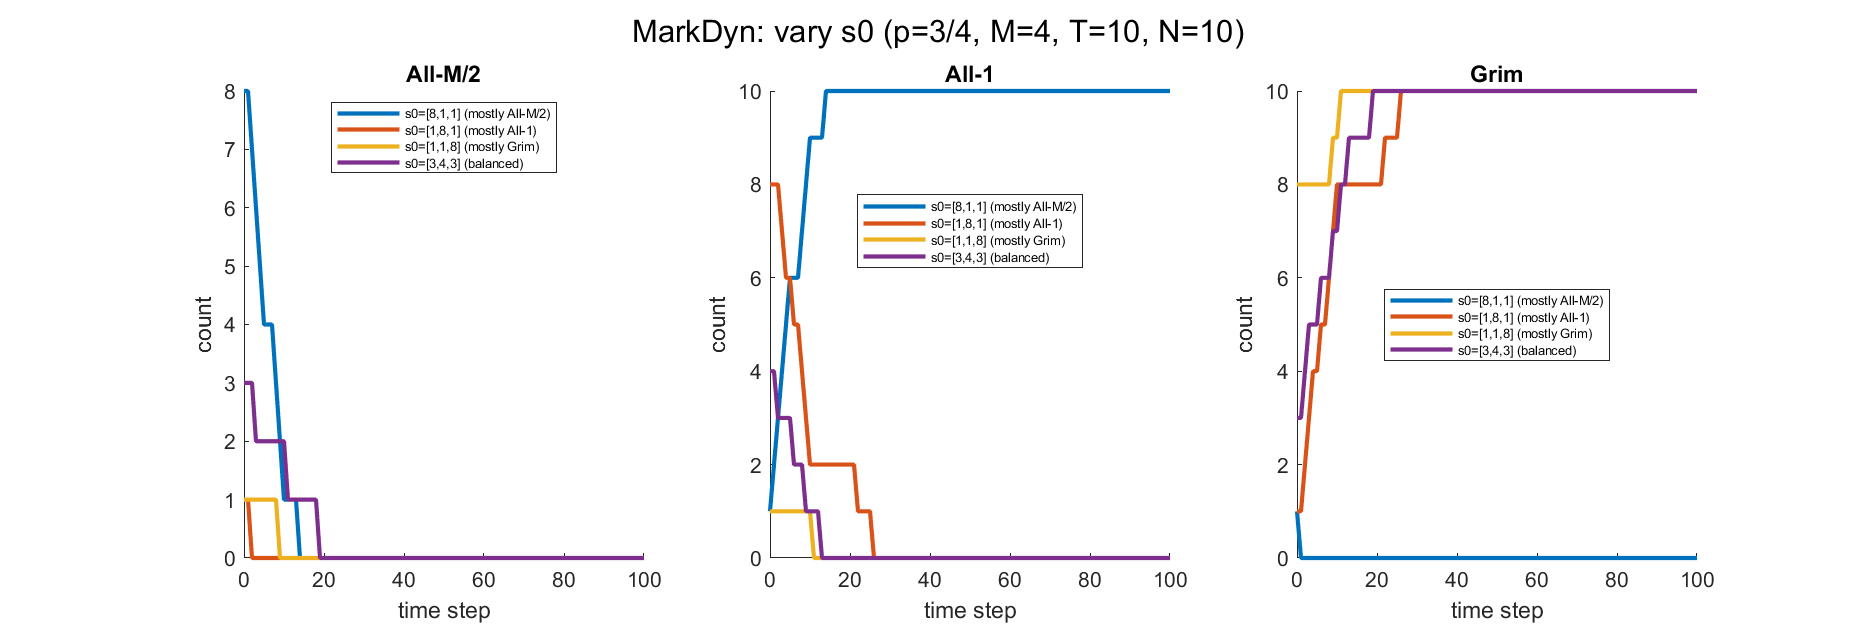
\includegraphics[width=\textwidth]{mark_overlay_vary_s0_p075}
  \caption{Markov dynamics: effect of varying initial state $s_0$
           ($p=3/4$, $M=4$, $T=10$, $N=10$).}
  \label{fig:mark_s0_p075}
\end{figure}

\begin{figure}[H]
  \centering
  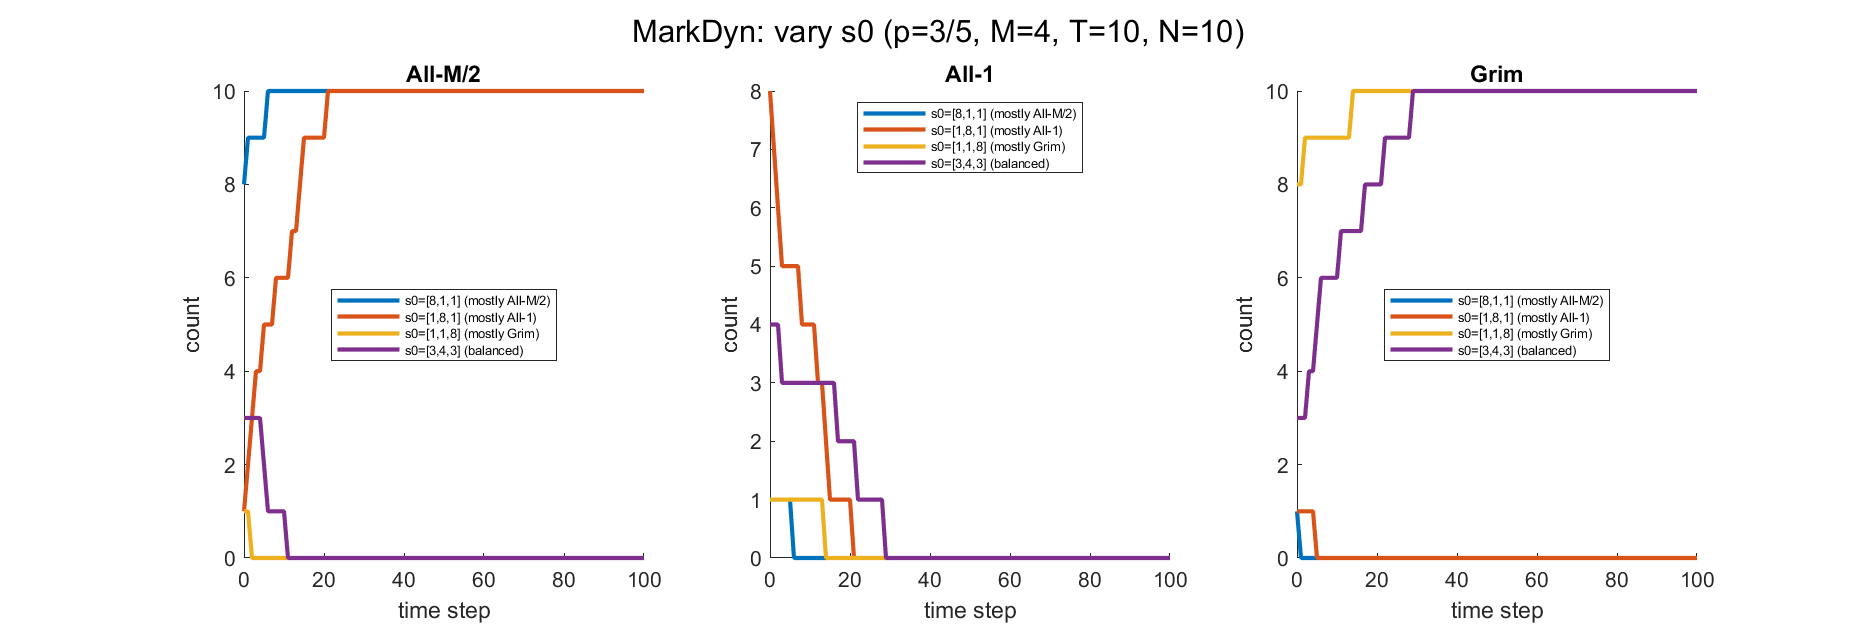
\includegraphics[width=\textwidth]{mark_overlay_vary_s0_p060}
  \caption{Markov dynamics: effect of varying initial state $s_0$
           ($p=3/5$, $M=4$, $T=10$, $N=10$).}
  \label{fig:mark_s0_p060}
\end{figure}

%=============================================================
\section{Connection to Learning Theory}
\label{sec:learning}
%=============================================================

Both evolutionary game theory (EGT) and learning models in games describe
adaptive behaviour in strategic environments and, as noted in~\cite{LK2026},
they generate identical dynamics under distinct interpretations.

In EGT, the population share $x_i(t)$ of strategy $i$ evolves via the
replicator dynamic
\[
  \dot{x}_i = x_i\bigl(\pi_i({\bf x})-\bar\pi({\bf x})\bigr),
  \qquad \bar\pi = \textstyle\sum_j x_j\pi_j({\bf x}).
\]
In learning models, individual agents adjust mixed strategies based on
reinforcement: the propensity $q_i$ to play action $i$ evolves as
$q_i(t+1) = q_i(t)+\alpha\pi_i(t)$, $x_i(t)=q_i(t)/\sum_j q_j(t)$.
It can be shown~\cite{BorgersSarin1997} that in large populations and
continuous time this rule converges to the replicator dynamic.

In the ISC context, this duality means:
\begin{itemize}
  \item \textbf{Evolutionary interpretation:} the fraction of players using
        Grim grows when Grim earns above-average payoffs; the stable outcomes
        (Grim dominance when $p>2/3$, or co-existence of All-$k$ and Grim
        separated by the threshold $p^*=M/6$) represent population-level
        selection pressures.
  \item \textbf{Learning interpretation:} individual players accumulate
        experience and shift probability toward more profitable strategies;
        Grim's superior payoff in self-play ($C(3,3)=TM$) means rational
        learners will reinforce cooperative reciprocal strategies over time.
\end{itemize}

%=============================================================
\section{Discussion}
\label{sec:discussion}
%=============================================================

\subsection{Effect of the All-\texorpdfstring{$M/2$}{M/2} Modification}

Table~\ref{tab:differences} summarises the structural differences between the
original paper (All-$M$) and this analysis (All-$M/2$).

\begin{table}[H]
\centering
\caption{Comparison: original paper (All-$M$) vs.\ this project (All-$M/2$).}
\label{tab:differences}
\small
\begin{tabular}{lll}
\toprule
Aspect & Original~\cite{LK2026} (All-$M$) & This work (All-$M/2$) \\
\midrule
Cooperator self-play payoff & $C(1,1)=TM=40$ & $C(1,1)=TM/2=20$ \\
Grim self-play payoff & $C(3,3)=TM=40$ & $C(3,3)=TM=40$ \\
Grim triggers vs cooperator & Never ($M\not<M$) & Always ($M/2<M$) \\
$s_2=0$ face absorbing? & Yes (entire face) & No \\
Absorbing states & $(0,N,0)$ + $s_2=0$ face & $(N,0,0)$, $(0,N,0)$, $(0,0,N)$ \\
Stable rest points (RD) & $s_2=0$ face + $(0,1,0)$ if $p>2/3$ & $(0,0,1)$ always; $(0,1,0)$ if $p>2/3$; $(1,0,0)$ if $p<M/6$ \\
Pure-Grim ESS & No (non-isolated set) & Yes (always) \\
\bottomrule
\end{tabular}
\end{table}

\subsection{The \texorpdfstring{$p = 2/3$}{p = 2/3} Threshold}

A critical threshold $p^*=2/3$ governs the stability of the all-defector state:
\begin{itemize}
  \item $p>2/3$ (e.g.\ $p=3/4$): $(0,1,0)$ is asymptotically stable
        (Propositions~\ref{prop:stab_allone},~\ref{prop:ESS_allone}).
        Both Grim and All-$1$ can be long-run outcomes.
  \item $p<2/3$ (e.g.\ $p=3/5$): $(0,1,0)$ is unstable. All-$1$ is driven out;
        the population converges to either pure Grim or (if $p$ is close
        to $2/3$) to pure All-$k$, separated by the unstable mixed rest point
        $x_1^*=(1+3p)/3$ on the All-$k$/Grim edge.
\end{itemize}
This threshold emerges identically in the modified game because the
payoffs against All-$1$ satisfy $C(1,2)=C(3,2)\approx T$ to leading order
(Grim and All-$k$ both receive approximately the same payoff against a pure
All-$1$ population), and the correction $C(3,2)-T=2-3p$ determines the sign.

\subsection{Grim Dominance}

Grim is the uniquely dominant strategy in self-play: $C(3,3)=TM=40$ vs.\
$C(1,1)=20$ and $C(2,2)=10$ for $M=4$, $T=10$. The modification amplifies
Grim's relative advantage: in the original paper All-$M$ matched Grim in
self-play ($C(1,1)=C(3,3)$), but here Grim earns twice as much. Analytically,
this is why the entire $s_2=0$ face ceases to be absorbing and $(0,0,1)$ becomes
the unique strictly dominant ESS.

%=============================================================
\section{Conclusion}
\label{sec:conclusion}
%=============================================================

This work has derived a complete game-theoretic and evolutionary analysis of the
ISC game with the strategy set $\{\text{All-}M/2, \text{All-}1, \text{Grim}\}$.
The main findings are:

\begin{enumerate}
  \item \textbf{Payoff matrix.} The ISC payoff matrix $C$ is analytically
        derived in closed form (Section~\ref{sec:C}), with numerical verification
        for $p\in\{3/4,3/5\}$, $M=4$, $T=10$.

  \item \textbf{Nash equilibria.} Three pure-strategy NE exist: $(0,0,1)$ always,
        $(0,1,0)$ iff $p\geq 2/3$, and $(1,0,0)$ iff $p\leq M/6$. For $M=4$ the
        latter two share the threshold $p^*=2/3$. A mixed NE on the
        All-$k$/Grim edge exists and is unstable (Section~\ref{sec:NE}).

  \item \textbf{Replicator dynamics.} Pure Grim is always asymptotically stable;
        the other pure vertices are stable only in the respective $p$-regime.
        All interior rest points are unstable (Section~\ref{sec:rep}).

  \item \textbf{Evolutionary stability.} Pure Grim is the unique ESS that holds
        for all parameters; the other pure vertices are ESS only in their
        respective stability regimes (Section~\ref{sec:ESS}).

  \item \textbf{Markov chain dynamics.} Only the three pure vertices are
        absorbing. The $s_2=0$ face is no longer absorbing (unlike in~\cite{LK2026})
        because Grim strictly outperforms All-$k$ in self-play. The basins of
        attraction are characterised by an explicit separating line $\ell$
        (Section~\ref{sec:markov}).

  \item \textbf{Parameter sensitivity.} Higher $p$ promotes All-$1$ stability;
        higher $M$ and $T$ amplify Grim's payoff advantage. Initial conditions
        affect convergence speed but not the qualitative long-run outcome.
\end{enumerate}

%=============================================================
\begin{thebibliography}{9}
\bibitem{LK2026}
  I.~Lazaridis and A.~Kehagias,
  \textit{Iterated Symmetric Centipede: Learning and Evolutionary Games},
  March 2026.

\bibitem{Hofbauer1998}
  J.~Hofbauer and K.~Sigmund,
  \textit{Evolutionary Games and Population Dynamics},
  Cambridge University Press, 1998.

\bibitem{Sandholm2010}
  W.~H.~Sandholm,
  \textit{Population Games and Evolutionary Dynamics},
  MIT Press, 2010.

\bibitem{BorgersSarin1997}
  T.~B\"{o}rgers and R.~Sarin,
  ``Learning through reinforcement and replicator dynamics,''
  \textit{Journal of Economic Theory}, vol.~77, pp.~1--14, 1997.
\end{thebibliography}

\end{document}